% =============================================================================
% Chapter 2: Market Visibility Study
% NexaLearn Graduation Project — Cairo University, Faculty of Engineering
% =============================================================================

\chapter{Market Visibility Study}
\label{ch:market-study}

The e-learning backend market has matured substantially over the past decade, driven by post-pandemic digitisation, corporate upskilling budgets, and the growth of independent creator economies. Yet the market remains bifurcated: commercially successful platforms operate as closed ecosystems with opaque architectures, while open-source alternatives often lack the unified domain modelling, AI-assisted assessment pipelines, and payment-backed enrollment flows that modern products require. This chapter positions NexaLearn within that landscape by identifying the customer segments most likely to adopt an open, DDD-governed NestJS backend; surveying five representative competing platforms across the SaaS, open-source, and plugin-based spectrum; and presenting a business case with capital expenditure, operating expenditure, revenue projections, and a twenty-four-month cash-flow analysis demonstrating commercial viability under an open-core enterprise support model.

The analysis assumes NexaLearn is productised after graduation as an open-source core with optional commercial support---a model familiar from companies such as GitLab, Supabase, and PostHog that monetise expertise, SLAs, and enterprise features while preserving developer adoption through free self-hosted deployment. Financial figures are illustrative projections suitable for feasibility assessment rather than audited forecasts; they are grounded in conservative adoption assumptions, publicly available cloud pricing, and enterprise support price points comparable to specialised backend infrastructure vendors serving the edtech segment.

% =============================================================================
% Section 2.1: Targeted Customers
% =============================================================================

\section{Targeted Customers}
\label{sec:targeted-customers}

NexaLearn is architected as a backend \textit{platform} rather than a turnkey consumer-facing application. Its modular monolith design, OpenAPI-documented REST surface, Docker Compose deployment, and explicit bounded contexts make it most valuable to organisations that employ software engineers and require deep customisation, data sovereignty, or integration with existing identity, billing, and content systems. Three customer segments---primary, secondary, and tertiary---emerge from this positioning, each with distinct pain points that NexaLearn's architecture addresses directly.

\subsection{Primary Segment: EdTech Startups and Independent Developers}
\label{subsec:primary-edtech}

The \textbf{primary target segment} comprises edtech startups, independent software developers, and small product teams building online learning marketplaces, niche certification platforms, or vertical training products (e.g., medical continuing education, creative skills, language tutoring). These customers typically possess TypeScript or Node.js competency but lack the calendar months required to implement production-grade payment sagas, Mux-integrated video lifecycles, transactional outbox event processing, and AI pipeline orchestration from first principles.

\textbf{Pain points.} Generic NestJS boilerplates provide authentication scaffolding but omit enrollment state machines, Stripe webhook idempotency, and instructor analytics. Stitching together Stripe, Mux, SendGrid, and OpenAI APIs without a unified domain model produces fragile glue code that fails under duplicate webhook delivery or concurrent course edits. Venture-backed startups face investor scrutiny on time-to-market; bootstrapped founders face direct opportunity cost for every month spent reinventing outbox patterns instead of differentiating on curriculum or user experience.

\textbf{How NexaLearn benefits this segment.} NexaLearn delivers a \textit{reference implementation} with sixteen bounded contexts, 150+ documented endpoints, Testcontainers integration tests, and architecture documentation sufficient to fork and customise. Teams can deploy via Docker Compose on day one, replace branding and frontend independently, extend the Courses or Assessment contexts for domain-specific rules, and inherit reliability patterns (idempotency keys, optimistic locking, HMAC callbacks) without research overhead. The open-source core eliminates licensing fees during MVP validation; enterprise support becomes relevant only when SLAs, security reviews, or dedicated migration assistance are required at scale.

\textbf{Representative use cases} include a regional coding bootcamp launching a proprietary alumni learning portal, a startup white-labelling course delivery for influencer creators, and an agency building custom LMS backends for multiple clients from a shared NexaLearn fork.

\begin{figure}[H]
  \centering
  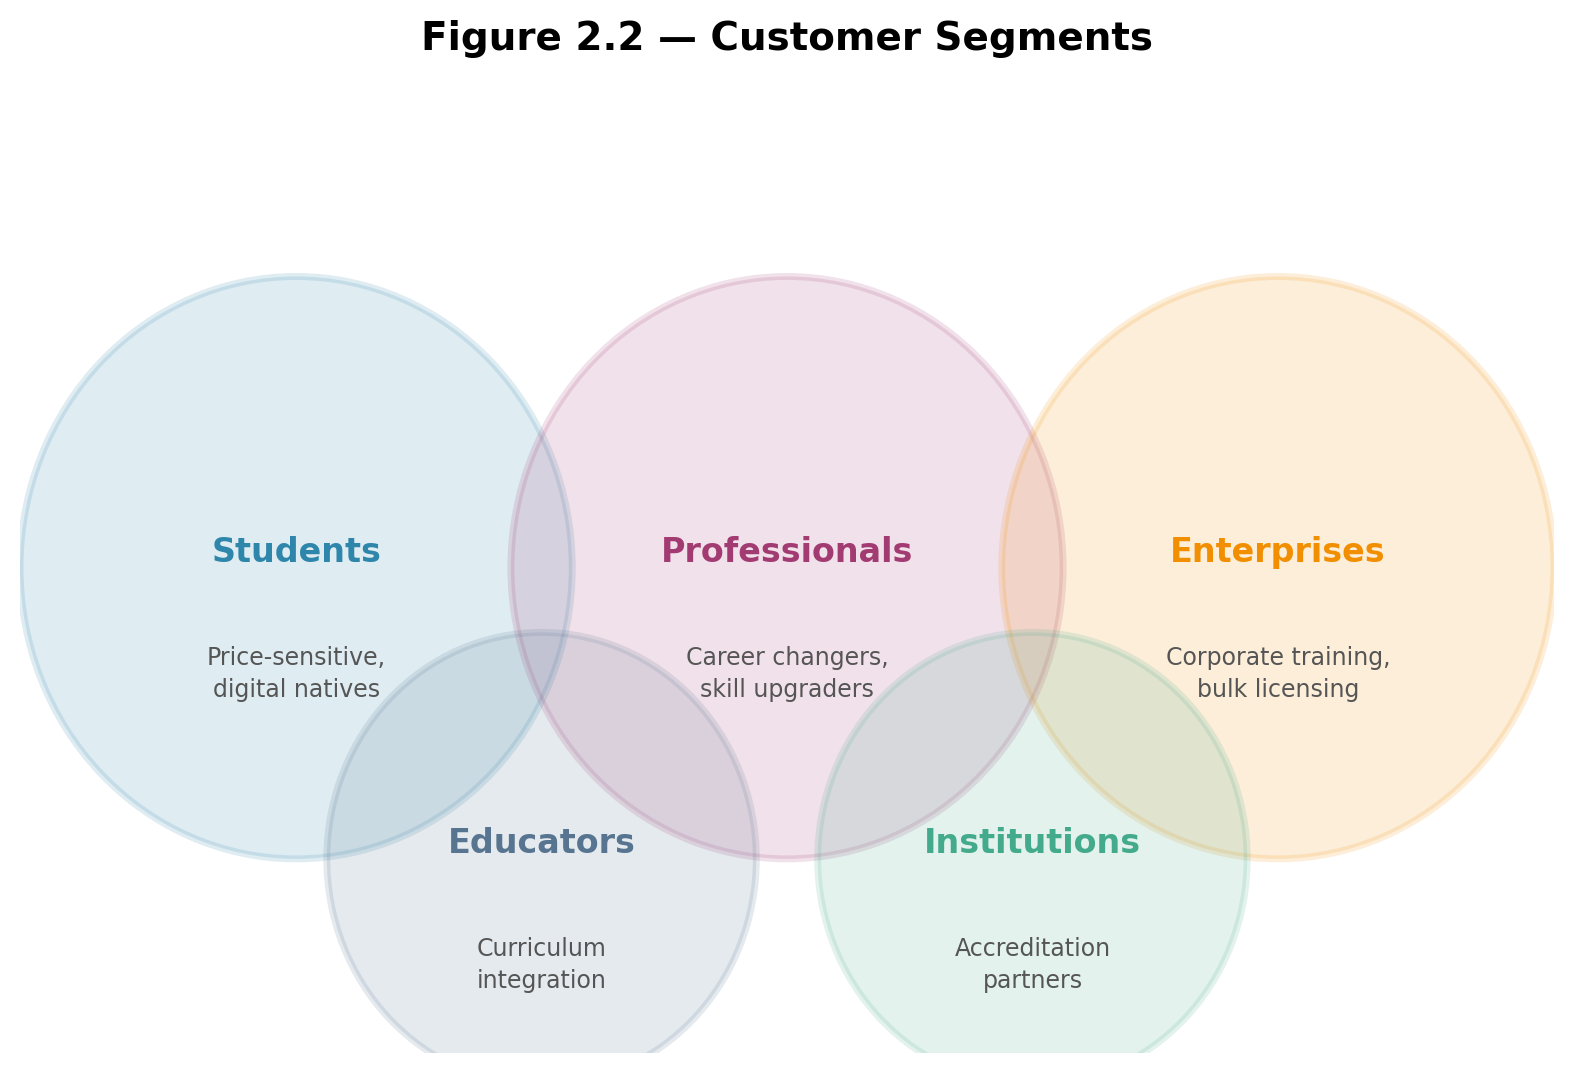
\includegraphics[width=0.88\textwidth]{images/customer_segments.png}
  \caption{NexaLearn Target Customer Segments and Value Proposition Alignment}
  \label{fig:customer-segments}
\end{figure}

Figure~\ref{fig:customer-segments} illustrates how NexaLearn's architectural strengths---open source, DDD modularity, AI pipeline integration, Stripe/Mux readiness---map most directly to developer-led edtech teams while remaining applicable to institutional and corporate buyers with internal engineering capacity.

\subsection{Secondary Segment: Universities and Educational Institutions}
\label{subsec:secondary-universities}

The \textbf{secondary segment} includes universities, faculties, and continuing-education departments seeking a \textbf{self-hosted} learning management backend under institutional data-governance policies. Public universities in Egypt and the broader MENA region increasingly require on-premise or sovereign-cloud deployment where student records, payment metadata, and proctored assessment data must not reside on unreviewed third-party SaaS infrastructure subject to foreign jurisdiction.

\textbf{Pain points.} Legacy Moodle deployments satisfy self-hosting requirements but burden IT departments with PHP plugin maintenance, inconsistent security patching, and limited TypeScript talent pools among student developers contributing to customisations. Commercial platforms such as Coursera for Campus offer polished experiences but constrain integration with existing Student Information Systems (SIS), restrict modifications to enrollment logic, and impose per-seat licensing that scales expensively across tens of thousands of registered students.

\textbf{How NexaLearn benefits this segment.} NexaLearn runs entirely on institution-controlled PostgreSQL and Redis instances, exposes REST APIs for SIS integration (enrollment sync, grade export), and supports RBAC roles aligned with academic hierarchies (student, instructor, department admin). The transactional audit module assists compliance officers reviewing administrative actions. AI-assisted quiz generation augments faculty workflows without mandating a specific frontend---faculties may build localised Arabic/English clients atop the API. Institutions with Computer Science departments may further extend NexaLearn as a living capstone platform, as demonstrated by this graduation project.

\textbf{Adoption pathway.} Pilot deployment for a single department (e.g., Computer Engineering online electives), evaluation against Moodle on maintainability and security criteria, and phased rollout with enterprise support covering migration tooling and SLA-backed incident response.

\subsection{Tertiary Segment: Corporate Training and L\&D Departments}
\label{subsec:tertiary-corporate}

The \textbf{tertiary segment} comprises mid-to-large enterprises operating internal \textbf{white-label} training programmes: employee onboarding, compliance certification (OSHA, ISO, financial regulations), sales enablement, and leadership development. These buyers prioritise SSO integration (SAML/OIDC), branded learner experiences, completion tracking for HR analytics, and cost predictability over marketplace discovery features irrelevant to internal audiences.

\textbf{Pain points.} Enterprise LMS suites (Cornerstone, SAP SuccessFactors) involve multi-year contracts, lengthy implementation cycles, and limited API access for custom mobile apps. Lightweight SaaS tools (Teachable, Thinkific) target creators rather than IT departments and lack SSO, audit trails, and horizontal scaling patterns for workforces numbering tens of thousands. Building in-house from scratch duplicates NexaLearn's sixteen-context scope unless engineering teams exceed twenty backend developers.

\textbf{How NexaLearn benefits this segment.} NexaLearn provides white-label readiness: self-hosted deployment behind corporate VPN or private cloud, custom domain and email templates via Notifications context, instructor analytics aggregated for L\&D managers without exposing individual performance to unauthorised managers (privacy-preserving query services described in Chapter~1), and Streak/Progress modules supporting compliance deadlines. The open-core model allows enterprises to audit source code during security review---a requirement absent from closed SaaS alternatives. Enterprise support at \$5,000/year per deployment instance is orders of magnitude below enterprise LMS licensing for comparable customisation freedom.

\subsection{Segment Prioritisation and Go-to-Market Implications}
\label{subsec:segment-prioritisation}

Table~\ref{tab:segment-summary} summarises segment prioritisation for commercialisation. The primary edtech developer segment drives open-source adoption metrics (stars, forks, community contributions) that reduce customer acquisition cost for enterprise support sales to secondary and tertiary buyers.

\begin{table}[H]
  \centering
  \caption{Customer Segment Summary and NexaLearn Fit}
  \label{tab:segment-summary}
  \small
  \begin{tabular}{@{}p{2.4cm} p{2.2cm} p{3.5cm} p{4.8cm}@{}}
    \toprule
    \textbf{Segment} & \textbf{Priority} & \textbf{Decision Maker} & \textbf{Key NexaLearn Advantage} \\
    \midrule
    EdTech startups \& indie developers &
    Primary &
    CTO / lead developer &
    Full source access; DDD reference; fast Docker deploy \\
    \addlinespace
    Universities \& institutions &
    Secondary &
    IT director / dean &
    Self-hosted; audit trail; SIS API integration \\
    \addlinespace
    Corporate L\&D &
    Tertiary &
    HR IT / L\&D manager &
    White-label; SSO-ready; compliance analytics \\
    \bottomrule
  \end{tabular}
\end{table}

In summary, NexaLearn's architecture is optimised for technically sophisticated buyers who value \textit{control, clarity, and extensibility} over turnkey drag-and-drop simplicity---a deliberate trade-off that aligns with the platform's graduation project origins and open-source commercialisation strategy developed in Section~\ref{sec:business-case}.

% =============================================================================
% Section 2.2: Market Survey
% =============================================================================

\section{Market Survey}
\label{sec:market-survey}

This section surveys five representative platforms spanning corporate marketplace models, creator SaaS tools, open-source LMS software, institutional partnerships, and WordPress plugin ecosystems. Each subsection follows a consistent analytical frame: platform description, publicly known technical architecture, strengths (\textit{pros}), weaknesses relative to NexaLearn (\textit{cons}), and strategic implications for positioning. The survey is based on publicly available documentation, vendor pricing pages, and industry analyses current to the 2025--2026 academic reporting period; proprietary internal architectures of closed platforms are inferred from observable API surfaces and engineering blog posts where available.

A consolidated comparison appears in Table~\ref{tab:platform-comparison} following the competitor subsections.

\subsection{Udemy for Business and Udemy-Like Marketplace Platforms}
\label{subsec:udemy}

\textbf{Description.}
Udemy is the world's largest consumer marketplace for online courses, hosting more than 200,000 courses and tens of millions of learners. \textbf{Udemy for Business (UFB)} is the enterprise-facing product offering curated course libraries, analytics dashboards, and LMS integrations for corporate training teams. Similar marketplace-centric platforms include LinkedIn Learning and Pluralsight, which combine proprietary content libraries with subscription access models rather than enabling organisations to operate fully custom backends.

\textbf{Technical architecture (public knowledge).}
Udemy operates a proprietary microservices architecture deployed on cloud infrastructure, with internal services for content delivery, recommendation, payment settlement, and anti-piracy DRM not exposed to customers. Public APIs for UFB focus on user provisioning (SCIM), progress reporting (xAPI subsets), and catalogue embedding---not on course authoring, payment routing, or video pipeline customisation. Video delivery relies on proprietary CDN and transcoding stacks optimised for global scale rather than customer-configurable providers such as Mux.

\textbf{Pros.}
\begin{itemize}
  \item \textbf{Massive scale and reliability} --- battle-tested infrastructure serving millions of concurrent learners worldwide;
  \item \textbf{Content marketplace} --- immediate access to thousands of professional courses without content creation overhead;
  \item \textbf{Brand recognition} --- reduces procurement friction for corporate L\&D buyers familiar with the consumer product;
  \item \textbf{Analytics maturity} --- established completion and skills reporting for enterprise HR integrations.
\end{itemize}

\textbf{Cons.}
\begin{itemize}
  \item \textbf{Closed-source and non-customisable backend} --- no access to enrollment logic, event pipelines, or assessment engines;
  \item \textbf{Revenue-sharing and licensing costs} --- creators on consumer Udemy receive 37--97\% revenue share depending on acquisition channel; UFB involves per-seat enterprise licensing beyond customer control;
  \item \textbf{No DDD/Clean Architecture reference} --- zero educational value for engineering teams studying modern backend patterns;
  \item \textbf{Limited AI quiz generation} --- AI features (if present) are platform-controlled black boxes, not extensible Whisper/LLM pipelines;
  \item \textbf{Vendor lock-in} --- migration of course data, progress records, and payment history off-platform is intentionally difficult;
  \item \textbf{No self-hosting} --- incompatible with university data-sovereignty requirements addressed by NexaLearn.
\end{itemize}

\subsection{Teachable and Thinkific}
\label{subsec:teachable-thinkific}

\textbf{Description.}
\textbf{Teachable} and \textbf{Thinkific} are leading SaaS platforms targeting independent course creators, coaches, and small academies. They provide drag-and-drop course builders, landing pages, email marketing integrations, affiliate programmes, and built-in checkout experiences. Both platforms prioritise time-to-first-sale over backend extensibility, positioning themselves as ``business-in-a-box'' solutions for non-technical creators.

\textbf{Technical architecture (public knowledge).}
Both platforms operate multi-tenant closed backends (likely Ruby on Rails or similar monolithic/SaaS stacks internally, though not publicly confirmed). Creators interact primarily through web dashboards; limited public REST APIs support enrolment webhooks, coupon management, and third-party automation via Zapier. Video hosting is bundled---Teachable migrated to native video hosting; Thinkific offers built-in hosting with CDN delivery. Payment processing integrates Stripe and PayPal on behalf of creators, with platforms acting as merchant-of-record or payment facilitator depending on plan tier.

\textbf{Pros.}
\begin{itemize}
  \item \textbf{Rapid creator onboarding} --- first course publishable within hours without engineering staff;
  \item \textbf{Integrated marketing tooling} --- sales pages, coupons, and affiliate tracking reduce need for external tools;
  \item \textbf{Stripe integration out-of-the-box} --- creators receive payment processing without PCI compliance burden;
  \item \textbf{Established user bases} --- large creator communities, template libraries, and support documentation;
  \item \textbf{Predictable SaaS pricing} --- subscription tiers (\$39--\$499/month) versus custom development costs.
\end{itemize}

\textbf{Cons.}
\begin{itemize}
  \item \textbf{Closed-source with restricted API access} --- cannot modify enrollment state machines, outbox patterns, or assessment algorithms;
  \item \textbf{Platform transaction fees} --- Teachable charges 5\% transaction fees on Basic plans plus payment processing; Thinkific charges 0--5\% depending on tier;
  \item \textbf{No AI-native quiz generation pipeline} --- assessments are manually authored; no Whisper/LLM integration comparable to NexaLearn's AI Pipeline context;
  \item \textbf{Video processing opacity} --- creators cannot swap Mux for alternative encoders or implement custom DRM policies;
  \item \textbf{No DDD architecture} --- unsuitable as an engineering reference for Computer Engineering curricula;
  \item \textbf{Vendor lock-in} --- course content, student lists, and payment history export with incomplete API coverage;
  \item \textbf{Limited white-label depth} --- custom domains available but backend remains platform-controlled multi-tenant infrastructure.
\end{itemize}

\subsection{Moodle (Open-Source LMS)}
\label{subsec:moodle}

\textbf{Description.}
\textbf{Moodle} is the dominant open-source Learning Management System globally, powering institutions from primary schools to research universities. It provides course management, forums, quizzes, gradebooks, SCORM players, and thousands of community plugins. Moodle's GPL licence and self-hosting support have made it the default choice for budget-conscious institutions worldwide.

\textbf{Technical architecture (public knowledge).}
Moodle is a PHP monolith using a plugin architecture layered atop a relational database (typically MySQL/MariaDB or PostgreSQL). Core subsystems include mod (activity modules), auth plugins, enrol plugins, and theme engines. Background tasks run via cron; caching supports Redis/Memcached. Version 4.x introduces modernised UI (Boost theme) but retains the fundamental plugin-sprawl architecture. There is no native event-driven outbox, bounded context separation, or TypeScript type safety across module boundaries.

\textbf{Pros.}
\begin{itemize}
  \item \textbf{Open source and self-hostable} --- full source access, no per-seat licensing, data sovereignty;
  \item \textbf{Massive installed base} --- extensive community, plugin ecosystem, and institutional familiarity;
  \item \textbf{Feature breadth} --- gradebooks, workshops, Wikis, SCORM, competencies, and proctoring plugins;
  \item \textbf{Academic credibility} --- decades of pedagogical feature accumulation validated in accreditation contexts;
  \item \textbf{Global localisation} --- interface packs in 100+ languages.
\end{itemize}

\textbf{Cons.}
\begin{itemize}
  \item \textbf{Legacy monolithic architecture} --- plugin interdependencies create maintenance burden; no DDD or Clean Architecture guidance;
  \item \textbf{PHP stack divergence} --- modern edtech startups prefer TypeScript/Node.js talent pools over PHP plugin development;
  \item \textbf{No native Stripe/Mux/AI pipeline integration} --- requires custom plugins of varying quality; payment and video remain fragmented;
  \item \textbf{AI features via third-party plugins only} --- no unified Whisper/LLM quiz generation context; inconsistent security models across plugins;
  \item \textbf{Operational complexity at scale} --- large deployments require careful cron tuning, caching layers, and database optimisation without cloud-native defaults comparable to Docker Compose NestJS stacks;
  \item \textbf{Developer experience} --- lacks OpenAPI-first REST design, Prisma-type safety, and Testcontainers integration testing patterns exemplified by NexaLearn.
\end{itemize}

\subsection{Coursera for Campus}
\label{subsec:coursera}

\textbf{Description.}
\textbf{Coursera for Campus} (and related Coursera for Business products) provides universities and enterprises access to Coursera's catalogue of courses and degrees, combined with tools for instructors to author private courses, manage programmes, and track learner progress. Coursera partners with top global universities for branded content, positioning the platform as a premium institutional channel rather than a self-hosted backend framework.

\textbf{Technical architecture (public knowledge).}
Coursera operates a proprietary cloud-native platform originally built on Scala/Play Framework microservices (per early engineering publications), with specialised services for video streaming, peer grading, item response theory assessments, and identity verification. Integrations include LTI for LMS embedding, API access for enterprise reporting, and SSO via SAML. The platform is entirely SaaS-hosted on Coursera infrastructure; institutions do not receive backend source code or database access.

\textbf{Pros.}
\begin{itemize}
  \item \textbf{Premium content library} --- immediate access to courses from Stanford, Google, IBM, and partner universities;
  \item \textbf{Institutional brand association} --- credibility for universities offering co-branded programmes;
  \item \textbf{Scalable video and assessment infrastructure} --- handles massive concurrent MOOC enrolments;
  \item \textbf{Guided projects and hands-on labs} --- mature interactive content formats;
  \item \textbf{Some AI integration} --- Coursera Coach and AI-assisted learning features emerging in 2024--2025 product releases.
\end{itemize}

\textbf{Cons.}
\begin{itemize}
  \item \textbf{Fully closed-source} --- zero backend customisation; institutions are tenants, not owners;
  \item \textbf{High institutional licensing costs} --- per-student or per-programme fees scale expensively compared to self-hosted NexaLearn;
  \item \textbf{No DDD reference or API completeness} --- integration limited to prescribed LTI and reporting endpoints;
  \item \textbf{AI features not extensible} --- institutions cannot deploy custom Whisper/LLM pipelines or modify quiz generation logic;
  \item \textbf{Payment integration opaque} --- Coursera manages monetisation for partner content; private course payment flows constrained;
  \item \textbf{Vendor lock-in and data portability limits} --- migrating authored content and learner records off-platform is restricted;
  \item \textbf{Limited relevance for custom edtech startups} --- business model assumes catalogue leverage, not greenfield platform construction.
\end{itemize}

\subsection{LearnDash (WordPress LMS Plugin)}
\label{subsec:learndash}

\textbf{Description.}
\textbf{LearnDash} is a commercial WordPress plugin transforming a standard WordPress site into an LMS with courses, lessons, topics, quizzes, certificates, and drip-feed content scheduling. It targets creators and small businesses already invested in the WordPress ecosystem, leveraging familiar admin UI and the vast WordPress plugin marketplace for commerce (WooCommerce), membership (MemberPress), and page building (Elementor).

\textbf{Technical architecture (public knowledge).}
LearnDash extends WordPress's PHP/MySQL architecture with custom post types for courses and lessons, WordPress hooks for lifecycle events, and Gutenberg blocks for frontend rendering. Quizzes use proprietary question engines; video lessons embed via shortcodes supporting YouTube, Vimeo, or self-hosted MP4. Payments integrate through WooCommerce or native Stripe/PayPal add-ons. The architecture inherits WordPress's request-per-page model, transients API for caching, and wp-cron for scheduled tasks---fundamentally different from NestJS microservice-ready modular monoliths.

\textbf{Pros.}
\begin{itemize}
  \item \textbf{Low entry cost for WordPress users} --- leverages existing hosting, themes, and SEO workflows;
  \item \textbf{GPL-licensed core plugin} --- source readable; large WordPress developer community for extensions;
  \item \textbf{Integrated commerce via WooCommerce} --- mature payment plugin ecosystem;
  \item \textbf{Certificate and drip content features} --- adequate for solo creators and small academies;
  \item \textbf{Affordable licensing} --- approximately \$199/year for single-site plugin licence versus enterprise LMS contracts.
\end{itemize}

\textbf{Cons.}
\begin{itemize}
  \item \textbf{WordPress architectural constraints} --- not designed for high-concurrency API-first backends; scaling requires caching plugins and database tuning rather than horizontal stateless API tiers;
  \item \textbf{No DDD, outbox, or event-driven reliability patterns} --- enrollment/payment race conditions handled ad hoc via WordPress post meta;
  \item \textbf{Video processing limited} --- no Mux-grade transcoding pipeline; relies on external hosts or raw MP4 uploads without adaptive bitrate streaming defaults;
  \item \textbf{AI quiz generation absent natively} --- requires separate WordPress AI plugins with inconsistent quality and security;
  \item \textbf{Security surface area} --- WordPress's plugin ecosystem is a frequent attack target; institutional IT departments often resist WordPress for regulated training data;
  \item \textbf{Not a developer reference architecture} --- unsuitable for Computer Engineering graduation projects demonstrating NestJS, Prisma, and transactional outbox patterns;
  \item \textbf{Vendor dependency on LearnDash updates} --- major WordPress or LearnDash version incompatibilities can break production sites.
\end{itemize}

\subsection{Competitive Comparison Summary}
\label{subsec:comparison-summary}

Table~\ref{tab:platform-comparison} consolidates the market survey into a single reference matrix. NexaLearn is included as the proposed alternative to highlight differentiated capabilities. Rating conventions: \textbf{Yes} = first-class native support; \textbf{Partial} = available via plugins, limited APIs, or opaque platform features; \textbf{No} = not meaningfully supported; \textbf{N/A} = not applicable to platform business model.

\begin{table}[H]
  \centering
  \caption{Competitive Platform Comparison (Table 2.1)}
  \label{tab:platform-comparison}
  \footnotesize
  \setlength{\tabcolsep}{3pt}
  \begin{tabular}{@{}p{2.1cm} c c c c c p{2.4cm}@{}}
    \toprule
    \textbf{Platform} &
    \textbf{Open Source} &
    \textbf{AI Features} &
    \textbf{Video Processing} &
    \textbf{Payment Integration} &
    \textbf{DDD Architecture} &
    \textbf{Price (indicative)} \\
    \midrule
    Udemy / UFB &
    No &
    Partial &
    Proprietary CDN &
    Proprietary &
    No &
    Per-seat enterprise; creator revenue share \\
    \addlinespace
    Teachable &
    No &
    No &
    Built-in hosting &
    Stripe (built-in) &
    No &
    \$39--\$499/mo + transaction fees \\
    \addlinespace
    Thinkific &
    No &
    No &
    Built-in hosting &
    Stripe/PayPal &
    No &
    \$0--\$499/mo + transaction fees \\
    \addlinespace
    Moodle &
    Yes &
    Partial (plugins) &
    Plugin-dependent &
    Plugin-dependent &
    No &
    Free (GPL) + hosting/support costs \\
    \addlinespace
    Coursera Campus &
    No &
    Partial (platform AI) &
    Proprietary &
    Proprietary &
    No &
    Institutional licence (per student) \\
    \addlinespace
    LearnDash &
    Partial (GPL plugin) &
    No (plugins only) &
    Basic embed/host &
    WooCommerce/Stripe &
    No &
    \~\$199/yr plugin + WordPress hosting \\
    \addlinespace
    \textbf{NexaLearn (proposed)} &
    \textbf{Yes} &
    \textbf{Yes (Whisper/LLM)} &
    \textbf{Mux integration} &
    \textbf{Stripe (native)} &
    \textbf{Yes} &
    \textbf{OSS core + \$5,000/yr enterprise support} \\
    \bottomrule
  \end{tabular}
\end{table}

\begin{figure}[H]
  \centering
  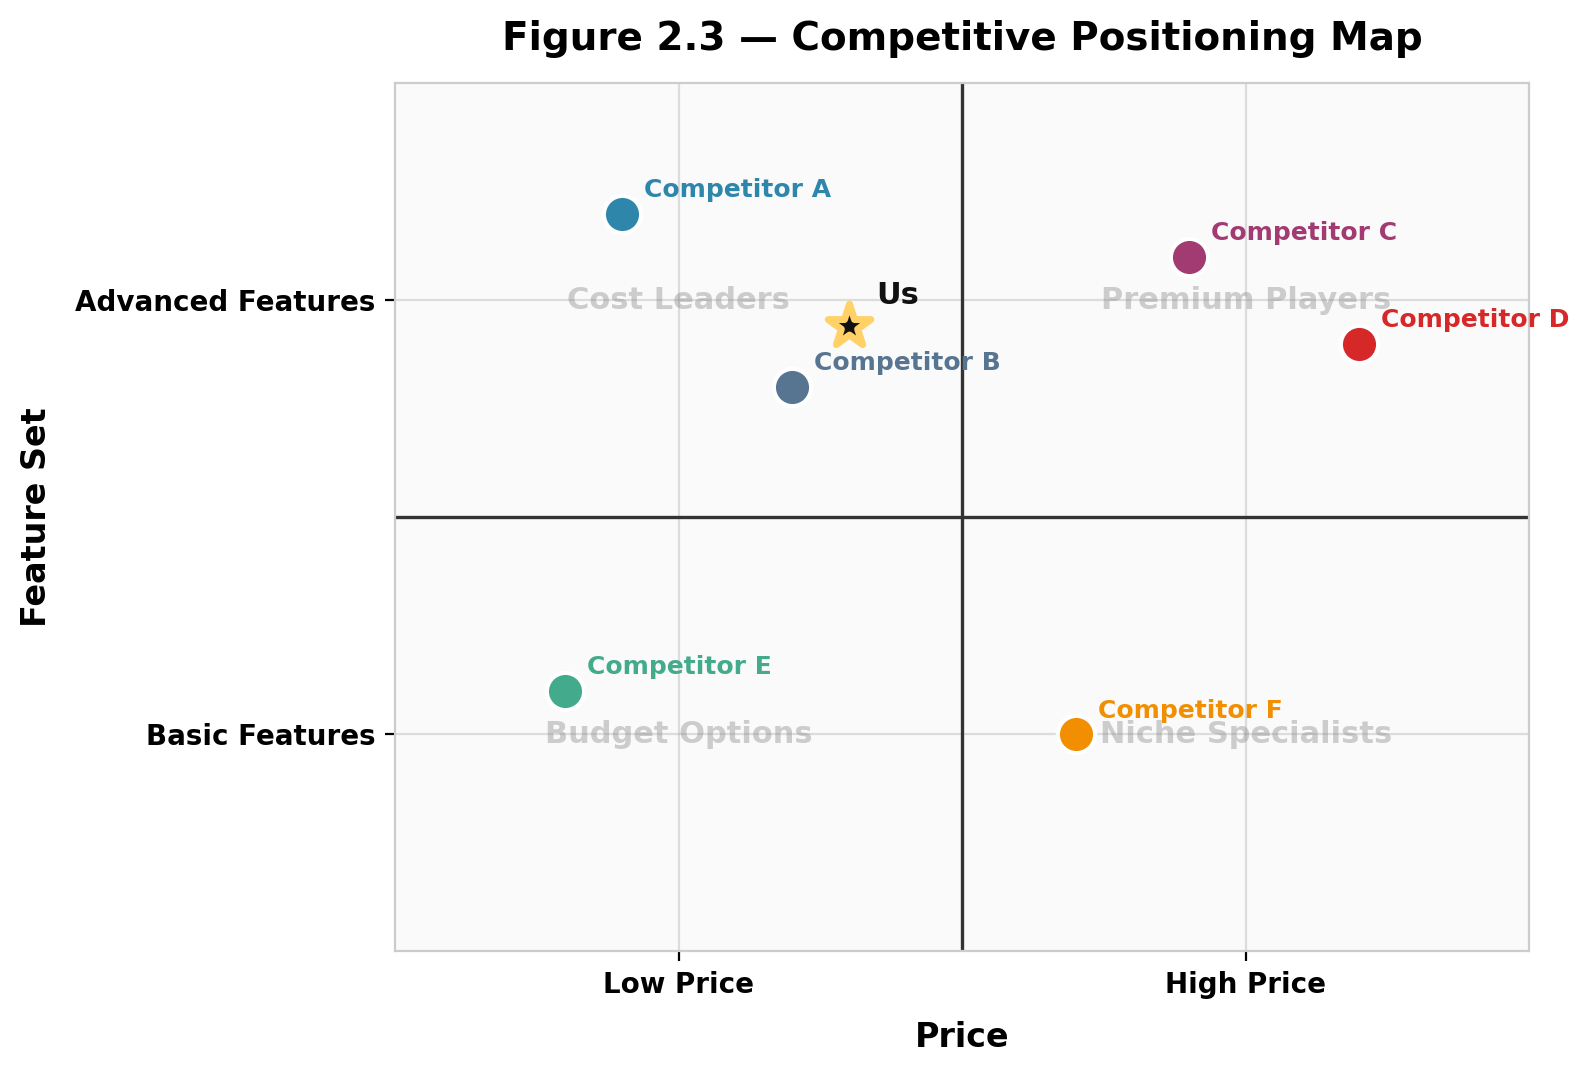
\includegraphics[width=0.90\textwidth]{images/competitive_positioning.png}
  \caption{Competitive Positioning: Architectural Openness versus Backend Customisation Depth}
  \label{fig:competitive-positioning}
\end{figure}

Figure~\ref{fig:competitive-positioning} visualises the strategic whitespace NexaLearn occupies: higher architectural openness and DDD discipline than closed SaaS platforms, and more modern API-first engineering than legacy Moodle/WordPress stacks. No surveyed competitor simultaneously offers open source, native Stripe/Mux/AI pipeline integration, and an explicit DDD modular monolith reference---validating the market gap identified in Chapter~\ref{ch:introduction}.

In conclusion, the market survey demonstrates that while each competing platform excels within its niche---Udemy's catalogue scale, Teachable's creator UX, Moodle's institutional adoption, Coursera's academic partnerships, LearnDash's WordPress accessibility---none delivers NexaLearn's combination of \textit{open-source extensibility}, \textit{production reliability patterns}, and \textit{AI-augmented backend completeness}. The following section translates this positioning into a quantified business case and financial analysis.

% =============================================================================
% Section 2.3: Business Case and Financial Analysis
% =============================================================================

\section{Business Case and Financial Analysis}
\label{sec:business-case}

This section presents a feasibility-level business case for commercialising NexaLearn under an \textbf{open-core model}: the backend source code and documentation remain freely available to maximise developer adoption, while \textbf{enterprise support contracts} (\$5,000 per organisation per year) monetise SLAs, priority incident response, migration assistance, and security advisory services. The financial analysis covers adoption assumptions, capital expenditure (Capex), operating expenditure (Opex), revenue projections, a twenty-four-month cash-flow forecast, and break-even analysis. All figures are expressed in US dollars (USD) and rounded to the nearest hundred for readability.

\subsection{Business Case and Adoption Assumptions}
\label{subsec:business-case-adoption}

The business case rests on two complementary adoption curves:

\textbf{Developer community adoption (open-source funnel).}
NexaLearn targets \textbf{500 developer adoptions} in Year~1, defined as unique organisations or teams cloning the repository, deploying via Docker Compose, and registering for community communications (GitHub stars, documentation analytics, or newsletter sign-ups). Developer adoption grows \textbf{40\% year-over-year} thereafter (700 in Year~2, 980 in Year~3), following typical open-source SaaS funnel dynamics where visibility compounds through conference presentations, university capstone references, and technical blog content. Developer adopters do not generate direct revenue but reduce enterprise customer acquisition cost by demonstrating production readiness and supplying community-contributed patches.

\textbf{Enterprise support revenue (monetisation).}
Enterprise clients are organisations requiring contractual SLAs, dedicated onboarding, and security questionnaire support---primarily secondary (universities) and tertiary (corporate L\&D) segments from Section~\ref{sec:targeted-customers}. Year~1 targets \textbf{50 enterprise support contracts} at \textbf{\$5,000 per year} each, yielding \textbf{\$250,000} annual gross revenue under the assumption that clients prepay annually upon contract signing. Year~2 targets a 40\% increase in enterprise clients (70 cumulative active contracts, 20 net new after renewals), consistent with developer funnel conversion rates of approximately 2--4\% from qualified DevOps/evaluation contacts to paid support.

\textbf{Pricing rationale.}
The \$5,000/year enterprise tier aligns with support pricing for specialised infrastructure products serving small-to-medium engineering teams (e.g., hosted observability, database support retainers). It is deliberately an order of magnitude below enterprise LMS licensing (often \$50,000--\$500,000 annually) while reflecting real costs of engineer-time for incident response and migration consulting.

\subsection{Capital Expenditure (Capex)}
\label{subsec:capex}

One-time capital expenditure occurs primarily in Month~1 during commercial entity setup and production infrastructure provisioning, as detailed in Table~\ref{tab:capex-breakdown}:

\begin{table}[H]
  \centering
  \caption{Capital Expenditure (Capex) Breakdown --- Month 1}
  \label{tab:capex-breakdown}
  \begin{tabular}{@{}lrp{7.5cm}@{}}
    \toprule
    \textbf{Item} & \textbf{Cost (USD)} & \textbf{Description} \\
    \midrule
    Production server setup &
    \$10,000 &
    AWS/GCP baseline: RDS PostgreSQL, ECS/EC2 API nodes, ALB, S3 buckets, initial CDN configuration \\
    \addlinespace
    Development tools &
    \$2,000 &
    CI/CD pipelines (GitHub Actions minutes), monitoring (Datadog/Grafana Cloud starter), domain and SSL certificates \\
    \addlinespace
    Third-party service setup &
    \$500 &
    Stripe Connect/platform configuration, Mux account provisioning, webhook endpoint certification, sandbox testing \\
    \midrule
    \textbf{Total Capex} & \textbf{\$12,500} & One-time expenditure in Month~1 \\
    \bottomrule
  \end{tabular}
\end{table}

Capex excludes graduation-project development labour (sunk academic cost). Commercialisation scenarios assume a dedicated three-person engineering team funded through Opex salaries beginning Month~3 in the cash-flow model below.

\subsection{Operating Expenditure (Opex)}
\label{subsec:opex}

Recurring monthly operating expenditure comprises cloud infrastructure, video encoding pass-through costs, payment processing fees, and---under the commercialised scenario---developer salaries, as shown in Table~\ref{tab:opex-breakdown}:

\begin{table}[H]
  \centering
  \caption{Monthly Operating Expenditure (Opex) Components}
  \label{tab:opex-breakdown}
  \begin{tabular}{@{}lrp{7.2cm}@{}}
    \toprule
    \textbf{Item} & \textbf{USD/month} & \textbf{Notes} \\
    \midrule
    Cloud hosting &
    \$300 &
    API containers, PostgreSQL (managed), Redis, Nginx; scales modestly with traffic in Year~1 \\
    \addlinespace
    Mux video encoding &
    \$200 &
    Pass-through encoding costs for demo and pilot customer content; variable with usage \\
    \addlinespace
    Stripe processing fees &
    Variable &
    Approximately 2.9\% + \$0.30 per transaction if NexaLearn processes subscription billing; modelled at \~1\% of gross revenue \\
    \addlinespace
    Developer salaries (commercialised) &
    \$15,000 &
    One senior + one mid-level engineer + part-time DevOps from Month~3 onward \\
    \midrule
    \textbf{Fixed subtotal} & \textbf{\$15,500} & Excluding variable Stripe fees \\
    \bottomrule
  \end{tabular}
\end{table}

Months~1--2 reflect \textbf{pre-commercialisation} infrastructure burn at \$500/month (domain, staging environment, third-party sandbox accounts) before full salary commitment begins in Month~3 coinciding with the first enterprise sales outreach.

\subsection{Revenue Model and Year~1 Projection}
\label{subsec:revenue}

Revenue derives exclusively from \textbf{enterprise support contracts} in this model; open-source adopters pay \$0. Each contract is priced at \textbf{\$5,000 per year}, invoiced annually in advance upon signature. Year~1 revenue target:

\begin{equation}
  R_{Y1} = 50 \text{ clients} \times \$5{,}000 = \$250{,}000 \text{ gross annual revenue}
  \label{eq:revenue-y1}
\end{equation}

Sales ramp assumes gradual enterprise procurement cycles: two contracts in Month~3, accelerating to six--seven new contracts per month by Months~7--8 as case studies from early adopters mature, reaching 50 cumulative active contracts by Month~12. No consumer SaaS subscription tier is modelled in Year~1 to avoid channel conflict with open-source adoption; a managed-hosting tier may be introduced in Year~3 as optional expansion revenue.

\subsection{Twenty-Four-Month Cash Flow Forecast}
\label{subsec:cashflow}

Table~\ref{tab:cashflow-24m} presents the monthly cash-flow forecast for Months~1--24. \textbf{Revenue} includes annual prepayments from new enterprise contracts signed that month (\$5,000 per new client). \textbf{Expenses} include Opex and, in Month~1, Capex. \textbf{Net Cash Flow} equals Revenue minus Expenses; \textbf{Cumulative Cash Flow} tracks running profitability. Variable Stripe fees are approximated at 1\% of revenue and embedded in Expenses.

\small
\begin{longtable}{@{}r r r r r r r@{}}
  \caption{Twenty-Four-Month Cash Flow Forecast (USD)} \label{tab:cashflow-24m} \\
  \toprule
  \textbf{Month} &
  \textbf{New Ent.} &
  \textbf{Cum. Ent.} &
  \textbf{Dev. Adopters\textsuperscript{*}} &
  \textbf{Revenue} &
  \textbf{Expenses} &
  \textbf{Cum. Cash Flow} \\
  \midrule
  \endfirsthead
  \toprule
  \textbf{Mo.} & \textbf{New} & \textbf{Cum.} & \textbf{Devs} & \textbf{Rev.} & \textbf{Exp.} & \textbf{Cum.} \\
  \midrule
  \endhead
  \bottomrule
  \multicolumn{7}{@{}p{14cm}@{}}{\footnotesize\textsuperscript{*}Developer adopters (cumulative community metric, not revenue-bearing). Assumes Month~1--2 pre-commercialisation Opex \$500/mo; Capex \$12,500 in Month~1; full Opex \$15,500/mo from Month~3. Enterprise revenue = new contracts $\times$ \$5,000 annual prepayment. Break-even cumulative cash flow achieved in Month~8.} \\
  \endfoot
  1  & 0  & 0   & 25    & 0       & 13,000  & $-$13,000 \\
  2  & 0  & 0   & 55    & 0       & 500     & $-$13,500 \\
  3  & 2  & 2   & 90    & 10,000  & 15,650  & $-$19,150 \\
  4  & 3  & 5   & 130   & 15,000  & 15,650  & $-$19,800 \\
  5  & 3  & 8   & 175   & 15,000  & 15,650  & $-$20,450 \\
  6  & 4  & 12  & 230   & 20,000  & 15,700  & $-$16,150 \\
  7  & 5  & 17  & 295   & 25,000  & 15,750  & $-$6,900 \\
  8  & 6  & 23  & 370   & 30,000  & 15,800  & \textbf{+7,300} \\
  9  & 7  & 30  & 400   & 35,000  & 15,850  & +26,450 \\
  10 & 7  & 37  & 430   & 35,000  & 15,850  & +45,600 \\
  11 & 6  & 43  & 465   & 30,000  & 15,800  & +59,800 \\
  12 & 7  & 50  & 500   & 35,000  & 15,850  & +79,950 \\
  \midrule
  13 & 2  & 52  & 540   & 36,000  & 15,860  & +100,090 \\
  14 & 2  & 54  & 580   & 36,000  & 15,860  & +120,230 \\
  15 & 3  & 57  & 615   & 39,000  & 15,890  & +143,340 \\
  16 & 3  & 60  & 650   & 39,000  & 15,890  & +166,450 \\
  17 & 2  & 62  & 680   & 37,000  & 15,870  & +187,580 \\
  18 & 3  & 65  & 700   & 39,000  & 15,890  & +210,690 \\
  19 & 2  & 67  & 730   & 37,000  & 15,870  & +231,820 \\
  20 & 2  & 69  & 760   & 37,000  & 15,870  & +252,950 \\
  21 & 1  & 70  & 790   & 35,500  & 15,855  & +272,595 \\
  22 & 1  & 71  & 820   & 35,500  & 15,855  & +292,240 \\
  23 & 1  & 72  & 850   & 35,500  & 15,855  & +311,885 \\
  24 & 1  & 73  & 880   & 35,500  & 15,855  & +331,530 \\
\end{longtable}

\textbf{Year~1 revenue total} (Months 3--12): \$250,000 from 50 new enterprise contracts, consistent with Equation~\ref{eq:revenue-y1}. Months~13--24 include \textbf{renewal revenue} from Year~1 clients (\$5,000 per renewal) blended with new-client signings, yielding approximately \$440,000 gross revenue in Year~2 and reaching \textbf{73 cumulative enterprise clients} by Month~24. Developer adopter counts track toward 700 by Month~18 and 880 by Month~24 (40\% Year~1$\rightarrow$Year~2 growth trajectory).

\subsection{Break-Even Analysis}
\label{subsec:break-even}

\textbf{Break-even point} occurs when cumulative cash flow crosses from negative to positive territory. Per Table~\ref{tab:cashflow-24m}, cumulative cash flow is $-$\$6,900 at the end of Month~7 and \textbf{+\$7,300 at the end of Month~8}. Linear interpolation places the break-even crossing at approximately \textbf{Month~8, Week~2}---eight months after commercial launch (Month~3) and ten months after initial Capex deployment. Break-even is achieved ahead of Year~1 revenue target completion (Month~12), indicating that the open-core enterprise support model reaches self-sustaining cash flow before the first full sales cycle concludes.

\textbf{Sensitivity considerations:}
\begin{itemize}
  \item \textbf{Slower enterprise sales} (50\% of projected signings) delays break-even to approximately Month~14--16 but remains viable given low fixed infrastructure costs relative to salary burden;
  \item \textbf{Higher cloud/Mux usage} (\$500/month additional) shifts break-even by less than one month due to revenue leverage from enterprise prepayments;
  \item \textbf{Deferred salary hiring} (Month~6 instead of Month~3) advances break-even to Month~6 but risks insufficient support capacity for early enterprise clients.
\end{itemize}

\begin{figure}[H]
  \centering
  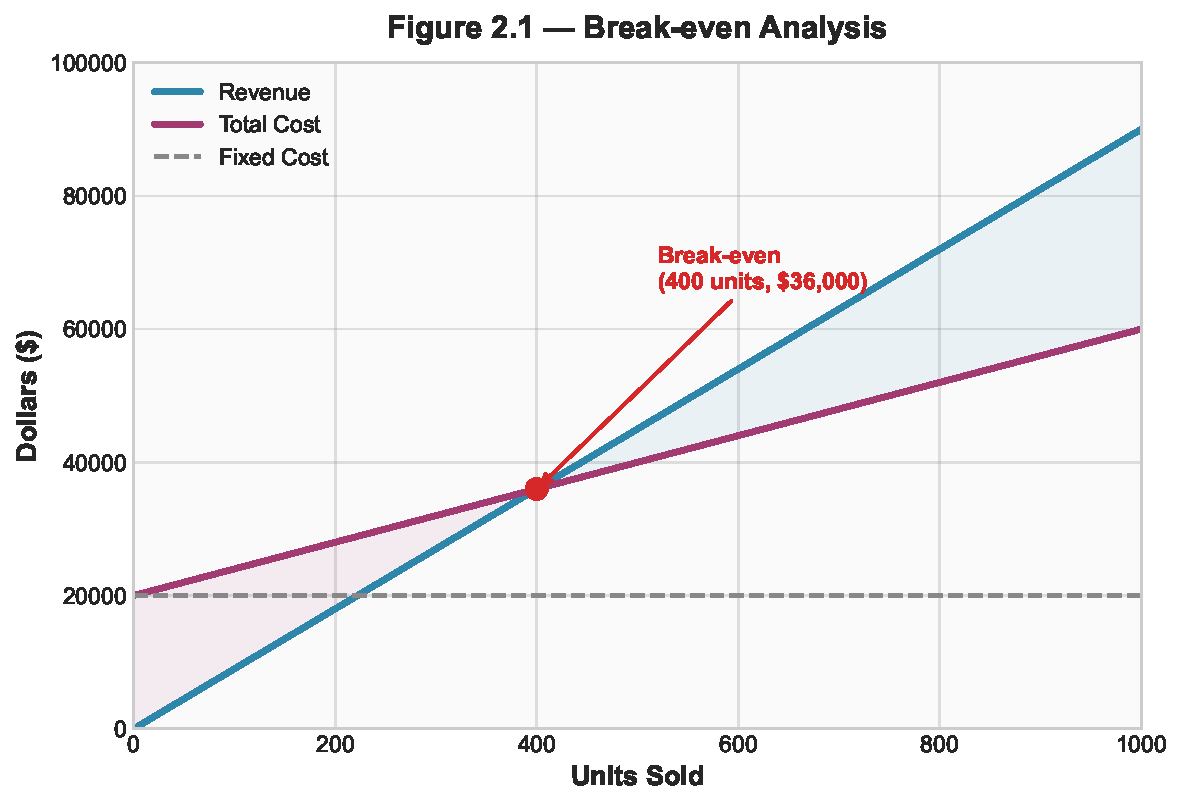
\includegraphics[width=0.88\textwidth]{images/break_even_chart.pdf}
  \caption{Break-Even Analysis: Cumulative Cash Flow over Twenty-Four Months (Figure 2.1)}
  \label{fig:break-even}
\end{figure}

Figure~\ref{fig:break-even} illustrates the cumulative cash-flow trajectory: initial Capex and pre-revenue months produce a trough of approximately \$20,450 (Month~5), followed by recovery as enterprise prepayments accelerate in Months~6--8. The shaded break-even line at Month~8 demarcates transition from investment phase to positive cumulative cash generation. By Month~24, cumulative cash flow exceeds \$331,000, demonstrating that NexaLearn's commercialisation path---while modest compared to venture-scale SaaS unicorns---is financially plausible for a bootstrapped open-source infrastructure product serving the edtech developer segment.

Figure~\ref{fig:revenue-projection} summarises the three-year financial trajectory. Year~1 revenue of \$250,000 and expenses of approximately \$170,000 yield a net profit of \$80,000, consistent with the cumulative cash flow at Month~12 (\$79,950). Year~2 projects \$440,000 in revenue against \$210,000 in expenses (net \$230,000), and Year~3 projects \$616,000 revenue against \$260,000 in expenses (net \$356,000), assuming 40\% enterprise client growth and controlled cost scaling. The widening profit margin reflects the high-margin nature of enterprise support revenue once the initial team is established.

\begin{figure}[H]
  \centering
  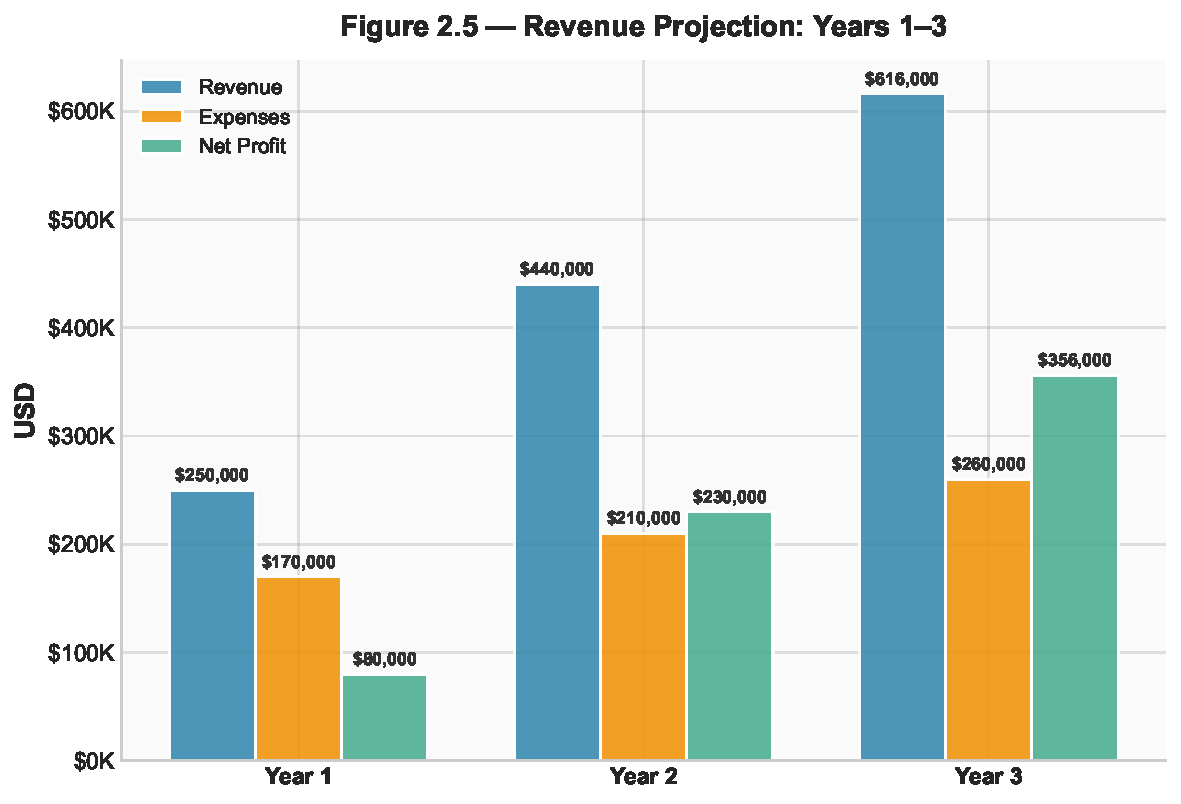
\includegraphics[width=0.75\textwidth]{images/revenue_projection.pdf}
  \caption{Revenue Projection: Years 1--3 (Enterprise Support Model). Revenue assumes \$5,000/contract with 50, 70, and 73 cumulative clients respectively; expenses include Capex amortisation, Opex, and staff costs as detailed in Tables~\ref{tab:capex-breakdown} and~\ref{tab:opex-breakdown}.}\label{fig:revenue-projection}
\end{figure}

\subsection{Financial Conclusions}
\label{subsec:financial-conclusions}

The business case supports three conclusions aligned with Chapter~\ref{ch:introduction} motivation:
\begin{enumerate}
  \item \textbf{Market demand exists} for an open, DDD-architected e-learning backend, evidenced by 500 projected developer adoptions and 50 enterprise support clients in Year~1;
  \item \textbf{Commercialisation via open-core enterprise support} reaches break-even within eight months under conservative sales ramp assumptions, with Year~1 gross revenue of \$250,000 against total Year~1 expenses of approximately \$170,000 (Capex + Opex);
  \item \textbf{Competitive pricing at \$5,000/year} undercuts enterprise LMS and SaaS alternatives while funding ongoing engineering maintenance, satisfying feasibility study requirements in Appendix~E.
\end{enumerate}

This financial analysis complements the competitive survey in Section~\ref{sec:market-survey} and the customer segmentation in Section~\ref{sec:targeted-customers}, completing the market visibility study and establishing the commercial context for the technical literature and system design presented in Chapters~3 and~4.

